
\documentclass[]{article}
\voffset=-1.5cm
\oddsidemargin=0.0cm
\textwidth = 480pt

% http://www.strath.ac.uk/aer/materials/5furtherquantitativeresearchdesignandanalysis/unit6/whatislogisticregression/

% http://www.medcalc.org/manual/logistic_regression.php


\usepackage{amsmath}
\usepackage{graphicx}
\usepackage{amssymb}
\usepackage{framed}
\usepackage{multicol}
%\usepackage[paperwidth=21cm, paperheight=29.8cm]{geometry}
%\usepackage[angle=0,scale=1,color=black,hshift=-0.4cm,vshift=15cm]{background}
%\usepackage{multirow}
\usepackage{enumerate}

%\SetBgScale{1}
%\SetBgAngle{0}
%\SetBgColor{black}
%\SetBgContents{\rule{1pt}{30cm}}
%\SetBgHshift{-8.4cm}
%
%\backgroundsetup{contents={
%\begin{tabular}{c|c}
%\hspace{2cm} & \\[0.7cm]
%& {\bf Statistics for Computing ------ Lecture 1 ------ Solutions} \\[0.3cm]
%%\hline
%\hspace{2cm} & \hspace{18.5cm} \\ [28cm]
%\end{tabular}}}





\begin{document}
\section*{Lab 2 Part C Independent t-test for two samples}

\section{Introduction}
The independent t-test, also called the \textbf{\textit{two sample t-test}} or  \textbf{\textit{independent-samples t-test}} or, is an inferential statistical test that determines whether there is a statistically significant difference between the means in two unrelated groups.

\subsection{Null and alternative hypotheses for the independent t-test}
The null hypothesis for the independent t-test is that the population means from the two unrelated groups are equal:

\[H_0: \mu_1 = \mu_2\]

\noindent In most cases, we are looking to see if we can show that we can reject the null hypothesis and accept the alternative hypothesis, which is that the population means are not equal:

\[H_1: \mu_1 \neq \mu_2\]

\noindent To do this, we need to set a significance level (also called \textit{alpha}) that allows us to either reject or accept the alternative hypothesis. Most commonly, this value is set at 0.05.

\subsection{What do you need to run an independent t-test?}
In order to run an independent t-test, you need the following:
\begin{itemize}
	\item One independent, categorical variable that has two levels/groups.
	\item One continuous dependent variable.
\end{itemize}


\subsection{Unrelated groups}

Unrelated groups, also called unpaired groups or independent groups, are groups in which the cases (e.g., participants) in each group are different. Often we are investigating differences in individuals, which means that when comparing two groups, an individual in one group cannot also be a member of the other group and vice versa. An example would be gender - an individual would have to be classified as either male or female – not both.

%------------------------------------------------%
\section{Assumption of normality of the dependent variable}
The independent t-test requires that the dependent variable is approximately normally distributed within each group.

\begin{framed}
\noindent \textbf{Note:} Technically, it is the residuals that need to be normally distributed, but for an independent t-test, both will give you the same result.
\end{framed}
\begin{itemize}
	\item You can test for this using a number of different tests, but the Shapiro-Wilks test of normality or a graphical method, such as a Q-Q Plot, are very common. You can run these tests using SPSS Statistics.
	\item However, the t-test is described as a robust test with respect to the Assumption of normality. This means that some deviation away from normality does not have a large influence on Type I error rates.
	\item The exception to this is if the ratio of the smallest to largest group size is greater than 1.5 (largest compared to smallest).
\end{itemize}


%------------------------------------------------%
\subsection{What to do when you violate the normality Assumption}
If you find that either one or both of your group's data is not approximately normally distributed and groups sizes differ greatly, you have two options: 
\begin{itemize}
	\item[(1)] transform your data so that the data becomes normally distributed. %%(to do this in SPSS Statistics see our guide on Transforming Data), or 
	\item[(2)] run the Mann-Whitney U test which is a non-parametric test that does not require the Assumption of normality. %% (to run this test in SPSS Statistics see our guide on the Mann-Whitney U Test).
\end{itemize}

%=========================================================%
\subsection*{Assumption of homogeneity of variance}
\begin{itemize}
	\item The independent t-test assumes the variances of the two groups you are measuring are equal in the population. If your variances are unequal, this can affect the Type I error rate. 
	\item The Assumption of homogeneity of variance can be tested using \textbf{\textit{Levene's Test of Equality of Variances}}, which is produced in SPSS Statistics when running the independent t-test procedure.
	\item  If you have run Levene's Test of Equality of Variances in SPSS Statistics, you will get a result similar to that below:
\end{itemize}

\begin{figure}[h!]
\centering
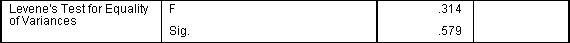
\includegraphics[width=0.5\linewidth]{TwoSample/Intro1}
\label{fig:intro1}
\end{figure}

%------------------------------------------------%
\subsection{Levene's Test for Equality of Variances in the Independent T-Test Procedure within SPSS}
This test for homogeneity of variance provides an F-statistic and a significance value (p-value). We are primarily concerned with the significance value – if it is greater than 0.05 (i.e., p $>$ .05), our group variances can be treated as equal. However, if p $< 0.05$, we have unequal variances and we have violated the 
Assumption of homogeneity of variances.

%------------------------------------------------%
\subsection{Overcoming a violation of the Assumption of homogeneity of variance}
\begin{itemize}
	\item If the \textbf{\textit{Levene's Test for Equality of Variances}} is statistically significant, which indicates that the group variances are unequal in the population, you can correct for this violation by not using the pooled estimate for the error term for the t-statistic, but instead using an adjustment to the degrees of freedom using the Welch-Satterthwaite method. 
	\item In all reality, you will probably never have heard of these adjustments because SPSS Statistics hides this information and simply labels the two options as ``\textbf{Equal variances assumed} and ``\textbf{Equal variances not assumed} without explicitly stating the underlying tests used. However, you can see the evidence of these tests as below:
\end{itemize}
\begin{figure}[h!]
\centering
\includegraphics[width=0.5\linewidth]{TwoSample/Ìntro2}

\label{fig:intro2}
\end{figure}

%------------------------------------------------%
\subsection{Differences in the t-statistic and the degrees of freedom when homogeneity of variance is not assumed}
\begin{itemize}
	\item From the result of Levene's Test for Equality of Variances, we can reject the null hypothesis that there is no difference in the variances between the groups and accept the alternative hypothesis that there is a statistically significant difference in the variances between groups. 
	\item The effect of not being able to assume equal variances is evident in the final column of the above figure where we see a reduction in the value of the t-statistic and a large reduction in the \textit{\textbf{degrees of freedom (df)}}. This has the effect of increasing the p-value above the critical significance level of 0.05. \item In this case, we therefore do not accept the alternative hypothesis and accept that there are no statistically significant differences between means. This would not have been our conclusion had we not tested for homogeneity of variances.
\end{itemize}

\newpage
%=========================================================%
\section{Reporting the result of an independent t-test}
\begin{itemize}
	\item When reporting the result of an independent t-test, you need to include the t-statistic value, the degrees of freedom (df) and the significance value of the test (p-value). 
	\item The format of the test result is: \texttt{t(df) = t-statistic}, \texttt{p = significance value}. 
	\item Therefore, for the example above, you could report the result as \texttt{t(7.001) = 2.233, p = 0.061}.
\end{itemize}


%------------------------------------------------%
\subsection{Fully reporting your results}
\begin{itemize}
	\item In order to provide enough information for readers to fully understand the results when you have run an independent t-test, you should include the result of normality tests, Levene's Equality of Variances test, the two group means and standard deviations, the actual t-test result and the direction of the difference (if any).
	\item  In addition, you might also wish to include the difference between the groups along with a 95\% confidence interval. For example:
\end{itemize}


%------------------------------------------------%
\begin{framed}
\begin{itemize}
	\item Inspection of Q-Q Plots revealed that cholesterol concentration was normally distributed for both groups and that there was homogeneity of variance as assessed by Levene's Test for Equality of Variances. 
	\item Therefore, an independent t-test was run on the data with a 95\% confidence interval (CI) for the mean difference. 
	\item It was found that after the two interventions, cholesterol concentrations in the dietary group (6.15 $\pm$ 0.52 mmol/L) were significantly higher than the exercise group (5.80 ± 0.38 mmol/L) (t(38) = 2.470, p = 0.018) with a difference of 0.35 (95\% CI, 0.06 to 0.64) mmol/L.
\end{itemize}
\end{framed}

%% To know how to run an independent t-test in SPSS Statistics, go to our SPSS Statistics guide here.

\newpage


%=========================================================%
\subsection*{Introduction}
\begin{itemize}
\item The independent-samples t-test (or independent t-test, for short) compares the means between two unrelated groups on the same continuous, dependent variable.
\item  For example, you could use an independent t-test to understand whether first year graduate salaries differed based on gender (i.e., your dependent variable would be "first year graduate salaries" and your independent variable would be ``nder", which has two groups: ``le" and ``male"). 
\item Alternately, you could use an independent t-test to understand whether there is a difference in test anxiety based on educational level (i.e., your dependent variable would be "test anxiety" and your independent variable would be ``ucational level", which has two groups: ``dergraduates" and ``stgraduates").
	
\item This  guide shows you how to carry out an independent t-test using SPSS Statistics, as well as interpret and report the results from this test.
\item However, before we introduce you to this procedure, you should understand the different Assumptions that your data must meet in order for an independent t-test to give you a valid result. We discuss these Assumptions later.
	
\end{itemize}

%------------------------------------------------%
%------------------------------------------------%

\section{Test Procedure in SPSS Statistics}
	In the section, Test Procedure in SPSS Statistics, we illustrate the SPSS Statistics procedure required to perform an independent t-test assuming that no Assumptions have been violated. First, we set out the example we use to explain the independent t-test procedure in SPSS Statistics.
	
	
	%------------------------------------------------%
\subsection{Cholesterol Example}
\begin{itemize}
\item 	The concentration of cholesterol (a type of fat) in the blood is associated with the risk of developing heart disease, such that higher concentrations of cholesterol indicate a higher level of risk, and lower concentrations indicate a lower level of risk. If you lower the concentration of cholesterol in the blood, your risk of developing heart disease can be reduced. 
\item Being overweight and/or physically inactive increases the concentration of cholesterol in your blood. Both exercise and weight loss can reduce cholesterol concentration. However, it is not known whether exercise or weight loss is best for lowering cholesterol concentration. \item Therefore, a researcher decided to investigate whether an exercise or weight loss intervention is more effective in lowering cholesterol levels. 
\item To this end, the researcher recruited a random sample of inactive males that were classified as overweight. This sample was then randomly split into two groups: Group 1 underwent a calorie-controlled diet and Group 2 undertook the exercise-training programme. 
\item In order to determine which treatment programme was more effective, the mean cholesterol concentrations were compared between the two groups at the end of the treatment programmes.
\end{itemize}

	
	%------------------------------------------------%
\subsection{Setup in SPSS Statistics}
	In SPSS Statistics, we separated the groups for analysis by creating a grouping variable called Treatment (i.e., the independent variable), and gave the "diet group" a value of "1" and the "exercise group" a value of "2" (i.e., the two groups of the independent variable). Cholesterol concentrations were entered under the variable name Cholesterol (i.e., the dependent variable). 
	
	%In our enhanced independent t-test guide, we show you how to correctly enter data in SPSS Statistics to run an independent t-test (see here). You can learn about our enhanced data setup content in general here. Alternately, we have a generic, "quick start" guide to show you how to enter data into SPSS Statistics, available here.
	
	%------------------------------------------------%
\subsection{Test Procedure in SPSS Statistics}
	The eight steps below show you how to analyse your data using an independent t-test in SPSS Statistics when the six Assumptions in the previous section, Assumptions, have not been violated. At the end of these eight steps, we show you how to interpret the results from this test. If you are looking for help to make sure your data meets Assumptions No.4, No.5 and No.6, which are required when using an independent t-test, and can be tested using SPSS Statistics, you can learn more here.
	
	Click Analyze > Compare Means > Independent-Samples T Test... on the top menu, as shown below:
	
\begin{figure}[h!]
\centering
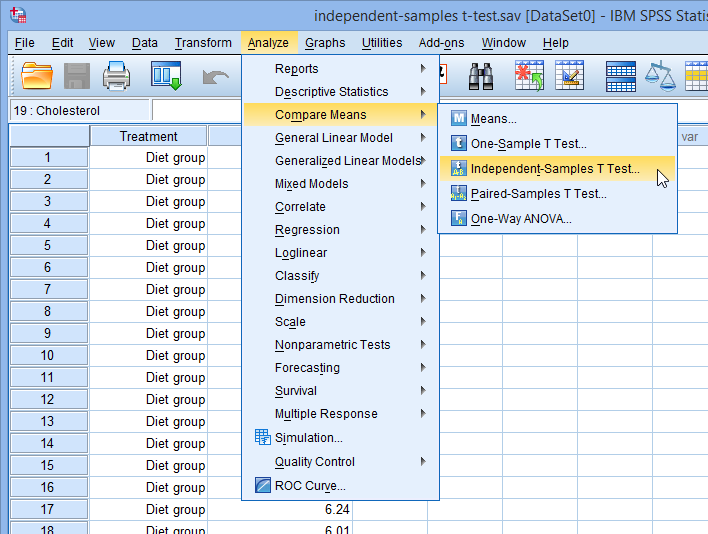
\includegraphics[width=0.5\linewidth]{TwoSample/TwoSampleMenu1}

\label{fig:TwoSampleMenu1}
\end{figure}\medskip

\noindent You will be presented with the Independent-Samples T Test dialogue box, as shown below:
	
\begin{figure}[h!]
	\centering
	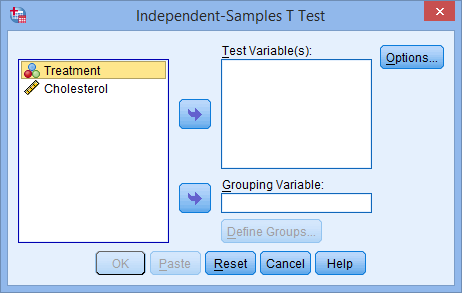
\includegraphics[width=0.5\linewidth]{TwoSample/TwoSampleMenu2}

	\label{fig:TwoSampleMenu2}
\end{figure}\medskip

\noindent Transfer the dependent variable, Cholesterol, into the Test Variable(s): box, and transfer the independent variable, Treatment, into the \texttt{Grouping Variable}: box, by highlighting the relevant variables and pressing the SPSS Right Arrow Button buttons. 
\newpage
You will end up with the following screen:
	
\begin{figure}[h!]
	\centering
	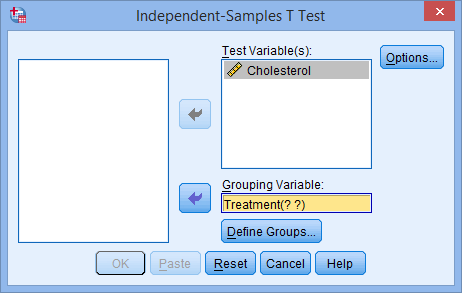
\includegraphics[width=0.35\linewidth]{TwoSample/TwoSampleMenu3}

	\label{fig:TwoSampleMenu3}
\end{figure}\medskip

\noindent You then need to define the groups (treatments). Click on the \texttt{Define Options} Button button. You will be presented with the \texttt{Define Groups} dialogue box, as shown below:
	
\begin{figure}[h!]
	\centering
	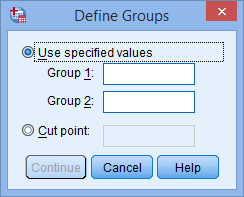
\includegraphics[width=0.35\linewidth]{TwoSample/TwoSampleMenu4}

	\label{fig:TwoSampleMenu4}
\end{figure}
\medskip

\noindent Enter ``1" into the Group 1: box and enter ``2" into the Group 2: box. Remember that we labelled the Diet Treatment group as 1 and the Exercise Treatment group as 2.
	
\begin{figure}[h!]
	\centering
	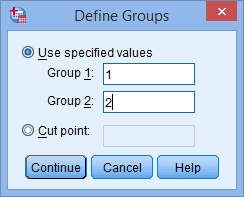
\includegraphics[width=0.5\linewidth]{TwoSample/TwoSampleMenu5}

	\label{fig:TwoSampleMenu5}
\end{figure}
\begin{framed}
	Note: If you have more than 2 treatment groups in your study (e.g., 3 groups: diet, exercise and drug treatment groups), but only wanted to compared two (e.g., the diet and drug treatment groups), you could type in 1 to Group 1: box and 3 to Group 2: box (i.e., if you wished to compare the diet with drug treatment).
\end{framed}	
	Click the \texttt{Continue} button.
	
	If you need to change the confidence level limits or change how to exclude cases, click the Options Button button. You will be presented with the following:
	
\begin{figure}[h!]
	\centering
	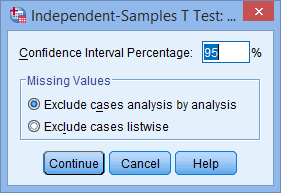
\includegraphics[width=0.5\linewidth]{TwoSample/TwoSampleMenu6}

	\label{fig:TwoSampleMenu6}
\end{figure}
	Click the \texttt{Continue} button. You will be returned to the \textit{Independent-Samples T Test} dialogue box. Then click the \texttt{OK} button.
	
	%------------------------------------------------%
	%------------------------------------------------%
\section{Output of the independent t-test in SPSS Statistics}
\begin{itemize}
	\item SPSS Statistics generates two main tables of output for the independent t-test. If your data passed Assumption No.4 (i.e., there were no significant outliers), Assumption No.5 (i.e., your dependent variable was approximately normally distributed for each group of the independent variable) and Assumption No.6 (i.e., there was homogeneity of variances), you will only need to interpret these two main tables. 
	
\item However, since you should have tested your data for these Assumptions, you will also need to interpret the SPSS Statistics output that was produced when you tested for them (i.e., you will have to interpret: (a) the boxplots you used to check if there were any significant outliers; (b) the output SPSS Statistics produces for your Shapiro-Wilk test of normality to determine normality; and (c) the output SPSS Statistics produces for Levene's test for homogeneity of variances). 

%If you do not know how to do this, we show you in our enhanced independent t-test guide here. 

\item Remember that if your data failed any of these Assumptions, the output that you get from the independent t-test procedure (i.e., the tables we discuss below) might not be valid and you might need to interpret these tables differently.
	
%\item However, in this "quick start" guide, we take you through each of the two main tables in turn, assuming that your data met all the relevant Assumptions.
\end{itemize}
	
	
\begin{figure}[h!]
\centering
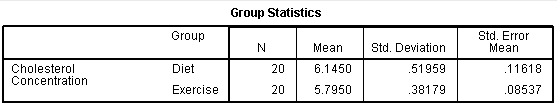
\includegraphics[width=0.7\linewidth]{TwoSample/TwoSampleOutpu1}

\label{fig:TwoSampleOutpu1}
\end{figure}

	This table provides useful descriptive statistics for the two groups that you compared, including the mean and standard deviation.
	

	Unless you have other reasons to do so, it would be considered normal to present information on the mean and standard deviation for this data. You might also state the number of participants that you had in each of the two groups. This can be useful when you have missing values and the number of recruited participants is larger than the number of participants that could be analysed.
	
	
	A diagram can also be used to visually present your results. For example, you could use a bar chart with error bars (e.g., where the error bars could use the standard deviation, standard error or 95\% confidence intervals). This can make it easier for others to understand your results.
	%% Again, we show you how to do this in our enhanced independent t-test guide.
	
	\newpage
\subsection{Independent Samples Test Table}
	This table provides the actual results from the independent t-test.
	
%	Output for the Independent T Test
%	Published with written permission from SPSS Statistics Inc., an IBM Company.
\begin{figure}[h!]
	\centering
	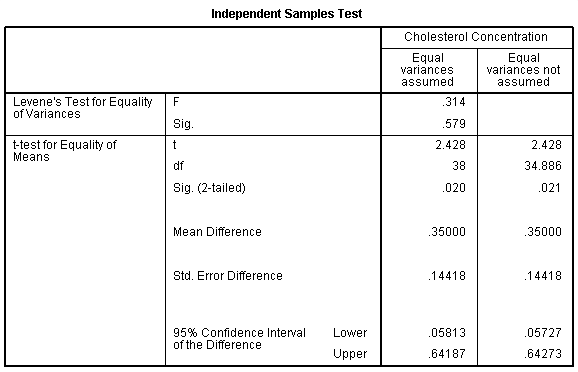
\includegraphics[width=0.6\linewidth]{TwoSample/TwoSampleOutput2}
	
	\label{fig:TwoSampleOutput2}
\end{figure}

	You can see that the group means are statistically significantly different because the value in the "Sig. (2-tailed)" row is less than 0.05. Looking at the Group Statistics table, we can see that those people who undertook the exercise trial had lower cholesterol levels at the end of the programme than those who underwent a calorie-controlled diet.
	
	%------------------------------------------------%
\subsection{Reporting the output of the independent t-test}
	Based on the results above, you could report the results of the study as follows (N.B., this does not include the results from your Assumptions tests or effect size calculations):
	
\subsection{General}
\begin{itemize}
	\item 	This study found that overweight, physically inactive male participants had statistically significantly lower cholesterol concentrations (5.80 $\pm$ 0.38 mmol/L) at the end of an exercise-training programme compared to after a calorie-controlled diet (6.15 $\pm$ 0.52 mmol/L), t(38) = 2.428, p = 0.020.
	
%%\item In our enhanced independent t-test guide, we show you how to write up the results from your Assumptions tests and independent t-test procedure if you need to report this in a dissertation, thesis, assignment or research report. 
%%We do this using the Harvard and APA styles (see here). 
\item It is also worth noting that in addition to reporting the results from your Assumptions and independent t-test, you are increasingly expected to report effect sizes.
% Whilst there are many different ways you can do this, we show you how to calculate effect sizes from your SPSS Statistics results in our enhanced independent t-test guide. 
\item Effect sizes are important because whilst the independent t-test tells you whether differences between group means are "real" (i.e., different in the population), it does not tell you the "size" of the difference. Providing an effect size in your results helps to overcome this limitation. 
%\item You can learn more about our enhanced independent t-test guide here, or our enhanced content in general here. If you use Stata rather than SPSS Statistics, we have a "quick start" guide on how to run an independent t-test here.
\end{itemize}

	
\section{Assumptions}
When you choose to analyse your data using an independent t-test, part of the process involves checking to make sure that the data you want to analyse can actually be analysed using an independent t-test. You need to do this because it is only appropriate to use an independent t-test if your data ``passes" six Assumptions that are required for an independent t-test to give you a valid result. In practice, checking for these six Assumptions just adds a little bit more time to your analysis, requiring you to click a few more buttons in SPSS Statistics when performing your analysis, as well as think a little bit more about your data, but it is not a difficult task.

Before we introduce you to these six Assumptions, do not be surprised if, when analysing your own data using SPSS Statistics, one or more of these Assumptions is violated (i.e., is not met). This is not uncommon when working with real-world data rather than textbook examples, which often only show you how to carry out an independent t-test when everything goes well! 

However, don't worry. Even when your data fails certain Assumptions, there is often a solution to overcome this. First, let's take a look at these six Assumptions:
\begin{description}
	\item[Assumption No.1:] Your dependent variable should be measured on a continuous scale (i.e., it is measured at the interval or ratio level). Examples of variables that meet this criterion include revision time (measured in hours), intelligence (measured using IQ score), exam performance (measured from 0 to 100), weight (measured in kg), and so forth.
	%% You can learn more about continuous variables in our article: Types of Variable.
	\item[Assumption No.2:] Your independent variable should consist of two categorical, independent groups. Example independent variables that meet this criterion include gender (2 groups: male or female), employment status (2 groups: employed or unemployed), smoker (2 groups: yes or no), and so forth.
	\item[Assumption No.3:] You should have independence of observations, which means that there is no relationship between the observations in each group or between the groups themselves. For example, there must be different participants in each group with no participant being in more than one group. This is more of a study design issue than something you can test for, but it is an important Assumption of the independent t-test. If your study fails this Assumption, you will need to use another statistical test instead of the independent t-test (e.g., a paired-samples t-test). 
	%%If you are unsure whether your study meets this Assumption, you can use our Statistical Test Selector, which is part of our enhanced content.
	
	\item[Assumption No.4:] There should be no significant outliers. 
	Outliers are simply single data points within your data that do not follow the usual pattern (e.g., in a study of 100 students' IQ scores, where the mean score was 108 with only a small variation between students, one student had a score of 156, which is very unusual, and may even put her in the top 1\% of IQ scores globally). The problem with outliers is that they can have a negative effect on the independent t-test, reducing the validity of your results. 
	
	Fortunately, when using SPSS Statistics to run an independent t-test on your data, you can easily detect possible outliers. 
	%In our enhanced independent t-test guide, we: (a) show you how to detect outliers using SPSS Statistics; and (b) discuss some of the options you have in order to deal with outliers. You can learn more about our enhanced independent t-test guide here.
	
	\item[Assumption No.5:] Your dependent variable should be approximately normally distributed for each group of the independent variable. We talk about the independent t-test only requiring approximately normal data because it is quite "robust" to violations of normality, meaning that this Assumption can be a little violated and still provide valid results. You can test for normality using the Shapiro-Wilk test of normality, which is easily tested for using SPSS Statistics. 
	%%In addition to showing you how to do this in our enhanced independent t-test guide, we also explain what you can do if your data fails this Assumption (i.e., if it fails it more than a little bit). Again, you can learn more here.
	\item[Assumption No.6:] There needs to be homogeneity of variances. You can test this Assumption in SPSS Statistics using Levene’s test for homogeneity of variances. 
	
	%%In our enhanced independent t-test guide, we (a) show you how to perform Levene’s test for homogeneity of variances in SPSS Statistics, (b) explain some of the things you will need to consider when interpreting your data, and (c) present possible ways to continue with your analysis if your data fails to meet this Assumption.
	
\end{description}
You can check Assumptions No.4, No.5 and No.6 using SPSS Statistics. Before doing this, you should make sure that your data meets Assumptions No.1, No.2 and No.3, although you don't need SPSS Statistics to do this. \\ \smallskip

\noindent When moving on to Assumptions No.4, No.5 and No.6, we suggest testing them in this order because it represents an order where, if a violation to the Assumption is not correctable, you will no longer be able to use an independent t-test (although you may be able to run another statistical test on your data instead).  \\ \smallskip

\noindent Just remember that if you do not run the statistical tests on these Assumptions correctly, the results you get when running an independent t-test might not be valid. \\ \smallskip

%%This is why we dedicate a number of sections of our enhanced independent t-test guide to help you get this right. You can find out about our enhanced independent t-test guide here, or more generally, our enhanced content as a whole here.

\end{document}
